The power subsystem is the as the name suggests the subsystem handling power for the Traffic Pi. Rather than pursuing a mobile power source of which size, duration of power, reliability, maintenance, and other characteristics play a part, the standard AC power cable that comes with a Raspberry Pi will be used to provide power to the entire system. 

\subsection{Power Cable}
The singular subsystem for the Power layer is the power cable for the Raspberry Pi. A power cable for connection to an AC wall outlet (5.1V micro USB supply) comes standard with most Raspberry Pi's. This subsystem will provide power to the Raspbery Pi which serves as the main computer "brain" for the Traffic Pi system.

\begin{figure}[h!]
	\centering
 	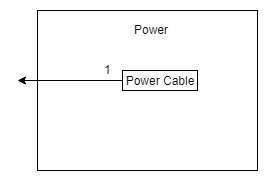
\includegraphics[width=0.60\textwidth]{images/power_layer}
 \caption{Power Layer}
\end{figure}

\subsubsection{Assumptions}
It is assumed that the 5.1V micro USB supply cable, when plugged into a standard US AC wall outlet will be able to supply sufficient Voltage to the Traffic Pi system (the Raspberry Pi, 3D camera, and IR camera) without strain or stress on either the system or power source.

\subsubsection{Responsibilities}
The power cable subsystem is responsible for providing sustained, constant, steady power for the Raspberry Pi that is part of the Traffic Pi system as a whole. 

\subsubsection{Subsystem Interfaces}
The power layer is unique in that it does not require a strict "interface" subsystem for communicating with the other layers in the Traffic Pi system. The power cable subsystem directly interfaces with the USB power supply socket on the Raspberry Pi.

\begin {table}[H]
\caption {Power cable subsystem interfaces} 
\begin{center}
    \begin{tabular}{ | p{1cm} | p{6cm} | p{3cm} | p{3cm} |}
    \hline
    ID & Description & Inputs & Outputs \\ \hline
    01 & 5.1V micro USB supply & \pbox{3cm}{N/A} & \pbox{3cm}{1 Amp}  \\ \hline
    \end{tabular}
\end{center}
\end{table}